\chapter{Origen}

\section{Origen histórico}

El origen de Scrum se remonta a la década del 80. La revista gerencial "Harvard Business Review" publica un artículo de Takeuchi y Nonaka denominado: "El nuevo nuevo juego para el desarrollo de productos" \cite{Takeuchi-Nonaka-1986}. En el artículo se describe cómo empresas tales como Honda, Canon y Fuji-Xerox producían nuevos productos a nivel mundial utilizando un enfoque diferente al tradicional de entonces. En ese artículo se introdujo el concepto Scrum, con el término tomado del deporte Rugby, para simbolizar este nuevo enfoque basado en equipos integrales para el desarrollo de productos. Hay autores que denominan a estos conceptos originales de Scrum como "Scrum pragmático" \cite{ScrumManager-2014}.

Una década más tarde, Jeff Sutherland y su equipo en Easel Corporation crearon el proceso de Scrum para ser utilizado en los procesos de 
desarrollo de software tomando los conceptos del artículo original de Takeuchi y Nonaka. Luego, en 1995, Jeff Sutherland junto con Ken Schwaber publican un informe sobre Scrum en una conferencia de Programación Orientada a Objetos OOPSLA. El informe fue formalizado con el nombre Proceso de Desarrollo SCRUM \cite{Ken-Schwaber-1995}. Hay autores que denominan a este marco de reglas para desarrollo de software como "Scrum técnico" \cite{ScrumManager-2014}. Desde esa fecha, Schwaber and Sutherland, han producido y publicado varias especificaciones para Scrum que han servido como guías y material de referencia; como por ejemplo: "Agile software development with Scrum" \cite{Ken-Schwaber-2002} y "The Scrum Guide" \cite{Ken-Jeff-2013}.

Luego, en los 90, Scrum paso a ser reconocidamente parte de las llamadas "Metodologías de Desarrollo de Software de peso liviano", junto a Crystal (1992), Feature Driven Development (1997), Desarrollo de Software Adaptativo (1999) y Extreme Programming (1999). Y luego del Manifiesto Ágil \cite{Beck-2001}, promulgado en 2001 y firmado por Ken y Jeff, pasó a ser reconocido como parte del movimiento ágil y su filosofía. Ken Schwaber fue el primer presidente de la Alianza Ágil fundada tras el Manifiesto Ágil.

Desde que surgió se popularizó en en el mundo industrial, principalmente en la industria de software, miles de proyectos en todo el mundo han utilizado Scrum para el desarrollo de productos, tanto en empresas pequeñas (startups) como en multinacionales. Debido a su amplia aplicación surgieron diferentes entidades capacitadoras y certificadoras para difundir Scrum y certificar el conocimiento de quienes rinden los respectivos exámenes necesarios. La Scrum Alliance \cite{Scrum-Alliance-2015} es un ejemplo de este tipo de organizaciones y es considerada la principal organización certificante. La Scrum Alliance fue fundada en 2002 por Ken Schwabe, Mike Cohn y Esther Derby. En 2006, Jeff Sutherland creó su propia compañía llamada Scrum.inc, sin dejar de ofrecer y enseñar a los cursos de Certified Scrum. A su vez, Ken dejó la Alianza Scrum en 2009 para fundar la Scrum.org para mejorar aún más la calidad y la eficacia de Scrum, principalmente a través de la serie Profesional Scrum ("Professional Scrum series"). Hay otras organizaciones capacitadoras y certificadoras como ScrumStudy que es una empresa (subsidiaria de VMEdu) que se basa en el libro "SBOK Guide" \cite{SBOK-2013}.

\section{Origen causal}

Scrum tuvo un origen causal que suele constituir el análisis crítico previo a su explicación. Scrum emerge del intento de resolver un problema y de la crítica a las consideradas causas del mismo. Scrum vino a surgir como una alternativa al modo en que se desarrollaba software y lo hizo como posible solución a los problemas que presentaba la situación en ese entonces (década del 90) de Desarrollo de Software. Por esa razón es que por lo general cuando se habla de Scrum se hace un análisis crítico previo para plantear un cambio debido a un problema. Por un lado, Scrum plantea un cambio paradigmático o filosófico que consiste en un cambio de perspectiva y de mentalidad (mindset). La otra cuestión fundamental es la metodológica en la cual se propone un cambio del proceso de desarrollo de software o proceso industrial de software. Por este motivo, para comenzar a comprender Scrum, hay que comprender cuál es el problema que viene a intentar resolver y qué es lo que se critica.

\subsection{Problema}

El problema principal por el que Scrum surgió como alternativa consistió en que la mayoría de los proyectos de desarrollo de software no lograban entregarse en tiempo, dentro de los costos y con las funcionalidades comprometidas. Ya en la primera conferencia organizada por la OTAN (en 1968) sobre desarrollo de software se hablaba de la "Crisis del Software" haciendo mención de los problemas recurrentes en que se veía afectado el desarrollo de software y sus resultados. En ese momento se identificaron entre diversos problemas la baja calidad del software que se desarrollaba, el no cumplimiento de las especificaciones y el código prácticamente inmantenible que dificultaba la gestión y la evolución de los proyectos. Una encuesta de cientos de proyectos de desarrollo de software empresarial indicó que cinco de seis proyectos de software se consideraban no satisfactorios \cite{AntiPatterns-1998}, por otro lado sólo 29 de cada 100 proyectos de IT se terminaban exitosamente y el 71 por ciento de los clientes no estaban satisfechos con los resultados (Standish Groups Chaos Report 1994 - 2004). En el año 1994 el Standish Group publicó un estudio conocido como el "CHAOS Report" \cite{CHAOS-Report-1994} donde se mostró las siguientes tasas de fracaso en los proyectos de desarrollo de software en general:

\begin{itemize}

\item \textbf{Proyectos cancelados:} el 31.1 por ciento es cancelado en algún punto durante el desarrollo del mismo.
\item \textbf{Proyectos insuficiente:} el 52.7 por ciento es entregado con sobrecostos, en forma tardía o con menos funcionalidades de las inicialmente acordadas.

%Las conclusiones de la investigación sugieren que el involucramiento del usuario y el empleo de periodos de tiempo más cortos son claves para incrementar las tasas de proyectos exitosos

\end{itemize}

\subsubsection{Causas}

Los problemas detectados en los modelos tradicionales se fundamentan principalmente en lo siguiente: 

\begin{itemize}

\item \textbf{Entorno cambiante:} Entorno altamente cambiante propio de la industria \cite{Martin-Alaimo-2014}.

\item \textbf{Dependencia de Procesos rígidos:} el proceso mismo de desarrollo de software donde el resultado depende de la actividad
cognitiva de las personas más que de las prácticas y controles de empleados \cite{Martin-Alaimo-2014}. Las metodologías de desarrollo de software resultaron muy pesadas y prohibitivas para responder satisfactoriamente a los cambios de negocio.

\end{itemize}

\subsection{Filosofía criticada}

Como se dijo antes, con Scrum se plantea un cambio paradigmático o filosófico que consiste en un cambio de perspectiva y de mentalidad (mindset). Algunas de las ideas que se critican son las siguientes:

\begin{itemize}

\item \textbf{Prevalencia de la opinión de expertos: }

La filosofía basada en expertos es una de las criticadas. Normalmente solemos favorecer la opinión de los expertos, pues consideramos que sólo una persona con experiencia y conocimientos es capaz de emitir juicios verdaderos o correctos en un área o materia en particular \cite{James-Surowiecki-2005}. Pues, es sabido que el juicio de expertos nos puede llevar a malos resultados debido, entre otras cosas, al "mecanismo de autoridad"\footnote{Mecanismo de autoridad: mecanismo por el cual uno se subordina a la opinión de un líder con autoridad o a un experto por su autoridad. El experimento de Milgram corrobora este fenómeno.} que hace que respetemos o sigamos las opiniones de los expertos aunque las mismas estén equivocadas.

\item \textbf{Cultura de Liderazgo: }
También se critica la filosofía basada en liderazgo que han generado gestión de control y mando. En el ámbito empresarial y en cierta época, ha prevalecido la filosofía del líder con gestión de control y mando. Podíamos ver una innumerable cantidad de ofertas de cursos de temáticas tales como, por ejemplo, "Masters en Liderazgo" y "Coaching en Liderazgo". Se tenía la idea de que si las organizaciones no eran fuertemente lideradas y los grupos humanos carecían de un líder entonces eran propensas al desastre. En esta perspectiva prevalecía la figura del líder coercitivo y transaccional. El líder coercitivo es el autoritario que se basa en la idea de jerarquía jefe y subordinado, y en la idea de mando y control. El líder transaccional es el que se basa en la motivación de premios y castigos, y también en la idea de negociación constante.

\item \textbf{Organizaciones centralizadas y jerárquicas: }
La idea del líder junto a la idea del control generan, entre otras cosas, la idea de la "jerarquía verticalista en organizaciones centralizadas". Idea que también se rechaza en el marco contextual de Scrum. Entre otras cosas, porque se genera una cultura donde prevalece el mecanismo de autoridad, mencionado anteriormente, y restringe la capacidad de innovación y creatividad. También puede generar sistemas culturales cerrados y rígidos ante situaciones cambiantes que requieren apertura y adaptación. En estas empresas de desarrollo de software, en la que se opera en base a la estandarización mecánica, pirámides de mando, estructuras jerárquicas, planificaciones estrictas y herramientas de control con la finalidad de controlar lo que acontece, controlando procesos y manipulando personas según planes, los planes fracasan con probabilidad alta.

\item \textbf{Cultura de la burocracia: } 
Las organizaciones centralizadas y jerárquicas pueden generar una cultura de la burocracia en la que se generan cargos y áreas que obstaculizan la ingeniería de requerimientos y en consecuencia al desarrollo de software. Mientras más personas intermedien entre el desarrollador y el cliente, más ruido se puede generar en las comunicaciones, generando así un desfase entre lo que el cliente realmente quiere y lo que se construye. Por ejemplo, si entre el desarrollador y el cliente se encuentran el analista de negocio, el encargado del producto, el ingeniero de aplicaciones y el jefe de ingeniería, es más probable que se forme el teléfono descompuesto en la cadena de comunicaciones y se termine construyendo un producto que no cumple las expectativas del cliente.

\item \textbf{Evaluación de desempeño individual: } 
Hace muchos años que una porción importante de los trabajadores, sociólogos y psicólogos viene expresándose en contra de las evaluaciones anuales de desempeño. Sin embargo, esa metodología sigue practicándose en las grandes organizaciones. En esas organizaciones, la cultura competitiva individualista fomenta el éxito individual en vez del colectivo y prevalece la cultura del sistemas de "evaluación de desempeño individual" en vez de grupal\footnote{Los métodos tradicionales de gestión de proyectos hacen hincapié en la responsabilidad individual hacia las responsabilidades del proyecto \cite{SBOK-2013}.}. Este tipo de sistema erosiona el trabajo colaborativo y de equipos necesario para trabajar con Agilidad. A pesar de los sistemas de premios y castigos en las organizaciones centralizadas y jerárquicas, los resultados siguen siendo diferentes a lo planificado. Por otro lado, los ciclos de retroalimentación para la evaluación de desempeño son ciclos largos que parecen no ser realmente útiles\footnote{Las empresas Deloitte y Accenture  comenzaron a desmantelar su engorrosa maquinaria de evaluación de desempeño. Pierre Nanterme, CEO de Accenture, dijo al Washington Post: "No estamos seguros de que todo el tiempo empleado en la gestión del rendimiento haya dado grandes resultados”, "Una vez al año les digo lo que pienso de ustedes. Eso no tiene sentido. La gente quiere saber... si lo está haciendo bien. Nadie va a esperar un ciclo anual para recibir esa retroalimentación” (Lucy Kellaway, 2015 The Financial Times Ltd.).}.

\end{itemize}

\subsection{Metodología criticada}

La causa de los problemas y fracasos de los proyectos de software en la situación dada, en ese entonces, de Desarrollo fueron atribuidos principalmente a la Metodología Cascada (Waterfall Methodology) \cite{Ken-Schwaber-1995}. Pero hay que tener en cuenta de qué se habla cuando se critica a la metodología cascada. Pues la metodología cascada no es el modelo cascada y en ocasiones se han atribuido, en un sentido erróneo, las causas de los problemas al modelo cascada. Pues no se puede comparar Scrum con el modelo Cascada porque Scrum no es exactamente un modelo y ofrece soluciones a aspectos que el modelo cascada no ofrece. Aunque sí, el modelo cascada, es parte de lo que se podría considerar una Metodología Cascada. 

\subsubsection{Modelo en Cascada}

El Modelo en Cascada (Waterfall Methodology) \cite{Ken-Schwaber-1995} es un Modelo Secuencial de Procesos para la ingeniería de software presentado por Winston Royce en 1970, aunque ya se venía desarrollando desde antes. Para algunos críticos, el Modelo en Cascada, se convirtió en el modelo metodológico más utilizado dentro de la industria en un período de tiempo. Pero hay que considerar que el modelo solo abarca al sistema de producción o sistema de desarrollo (ver "Development Process" en la figura \ref{fig:WaterfallMethodology}) de la industria, no al de gestión, y es simplemente un modelo, no una metodología.

\begin{figure}[h]
  \centering
  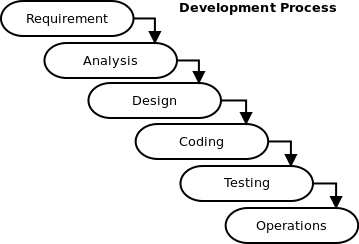
\includegraphics[width=0.75\textwidth]{WaterfallModel}
  \caption{Modelo Cascada de desarrollo}
  \centering
  \label{fig:WaterfallModel} %\ref{fig:WaterfallModel}
\end{figure}

En un sentido lato y ortodoxo se puede decir que el Modelo en Cascada refleja un proceso lineal y secuencial de un conjunto de procesos o fases independientes dentro de un proyecto. Las fases son: requerimientos (requerimiento del sistema y requerimientos del software), diseño, codificación, pruebas y operación. Según esto y siempre cuando el proceso de desarrollo de un proyecto conste de solo la secuencia de estas fases sin repetición, la principales críticas como desventajas que se hacen son:

\begin{enumerate}

\item \textbf{Previsión:} \newline
Si un proyecto tiene una fase de requerimientos única al comienzo, el producto final debe ser anticipado de antemano \cite{Scrum-Institute-2015} y esto requiere de cierta previsión y certidumbre inicial. La previsión es acorde a una mirada más tradicional y analitica que concidera que el diseño se puede planificar en detalle al comienzo del proceso de desarrollo. A este método y práctica se lo llama BMUF que significa “Diseño Inicial Grande” o "Gran Modelado al Inicio" y con él se establece la práctica de realización explícita de Diseño Arquitectónico Completo al Inicio \cite{Wiley-Sons-2002}. Es el mandato técnico de crear modelos integrales de los requisitos para un sistema, el análisis de esos requisitos, una arquitectura que cumple esos requisitos y, finalmente, un diseño detallado antes de implememtar el sistema. Lo que sucede es que cierta previsión y certidumbre inicial y necesaria, en proyectos complejos y cambiantes, es poco factible que suceda. Esto lo muestra el modelo del "cono de incertidumbre"\footnote{\cite{McConnell-2006}, \cite{Boehm-1981}, \cite{Martin-Alaimo-2014}} en la industria de software (ver figura \ref{fig:ConeOfUncertainty}) que indica que en la evolución de la incertidumbre a lo largo de un proyecto el nivel inicial se corresponde a un +- 400 por ciento y tiende a disminuir a lo largo del proyecto. Por tal motivo preveer el proyecto en su primera parte no es efectivo y tomar decisiones difíciles de cambiar en esa etapa no sería conveniente.

\begin{figure}[h]
  \centering
  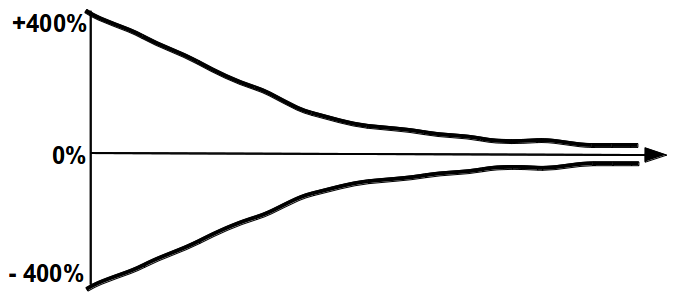
\includegraphics[width=0.60\textwidth]{ConeOfUncertainty}
  \caption{Cono de la incertidumbre en contextos inestables}
  \centering
  \label{fig:ConeOfUncertainty} %\ref{fig:ConeOfUncertainty}
\end{figure}

\item \textbf{Requerimientos no necesarios:} \newline
Cuando los requerimientos son elicitados al comienzo de un proyecto e implementados posteriormente, podrían nunca ser completamente necesitados por el cliente a partir del final del proyecto \cite{Scrum-Institute-2015}. O sea que pueden haber requerimientos irrelevantes o innecesariamente implementados, ya sea porque el cliente dejó de tener la necesidad en el transcurso del proyecto o porque la incertidumbre inicial generó una mala elicitación de los mismos.

\item \textbf{Fases separadas:} \newline
Cada fase es estrictamente separada \cite{Scrum-Institute-2015}. Por ejemplo una vez que se encuentra completa la fase de requerimientos se procede a una firma de aprobación o "sign-off" que congela dichos requerimientos, y es recién aquí cuando se puede iniciar la fase de diseño, fase donde se crea un plano de modelo o "blueprint" del mismo para que, luego, los programadores lo codifiquen, se prosiga con las pruebas y finalmente el despliegue en operación. Pues en entornos altamente cambiante, propio de la industria de software, esta forma secuencial estricta hace del proceso de desarrollo un proceso “pesadas” (estanco y burocrático) y prohibitivo para responder satisfactoriamente a los factores cambiantes de negocio \cite{Martin-Alaimo-2014}.
%Solución propuesta por scrum:
%Fine-grained requirements are only defined when they are really needed.
%All activities to design, build and test a certain functionality are kept together in one phase.
%Changes are expected and welcomed by Scrum team.

\end{enumerate}

\subsubsection{Gestión de Proyectos Clásica}

Bajo el marco Scrum se critica el uso de la gestión de proyectos tradicional o clásica (ver figura \ref{fig:PMIMethodology}) en proyectos de dominios complejos y con dinámica de requerimientos cambiantes. Se atribuye parte de los fracasos a las siguientes causas:

\begin{figure}[h]
  \centering
  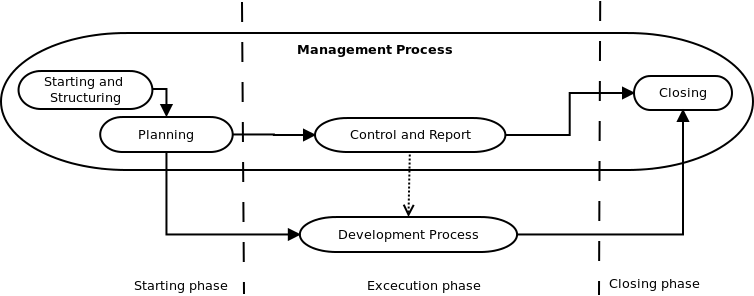
\includegraphics[width=0.99\textwidth]{PMIMethodology}
  \caption{Metodología de Gestión de Proyectos Clásica PMI}
  \centering
  \label{fig:PMIMethodology} %\ref{fig:PMIMethodology}
\end{figure}

\begin{enumerate}

\item \textbf{Planeación predictiva:} La planeación predictiva fue impulsada por el PMI quien ha adoptado el enfoque predictivo y mecanicista para la gestión de proyectos. Planeación predictiva es cuando el alcance del proyecto, el tiempo y el costo requerido para el proyecto se determina lo antes posible, en la fase de inicio del proyecto, y luego durante la ejecución del proyecto se busca seguir y respetar el plan hasta la fase de cierre (ver figura \ref{fig:PMIProject}). El éxito (o rendimiento) del enfoque predictivo ha sido menos del 50 por ciento (en tiempo, en la fecha y con la funcionalidad deseada) y Scrum se presenta como alternativa para mejorar esta tasa \cite{Ken-Schwaber-2011}. El enfoque predictivo es útil para producción de volumen alto y fabricación de bajo coste. Sus beneficios resultan de reducir la imprevisibilidad del espacio del problema a través de la estandarización y la repetición. La planificación perfecta, la formación y la repetibilidad son las claves. Planificar y luego hacer una y otra vez. La productividad se optimiza a través de procesos de flujo de trabajo perfecto e invariable, y se optimiza el uso de los recursos (personas o máquinas). Pero esta metodología no se ajusta a proyectos donde hay más novedad que repetibilidad y donde las tecnologías, capacidades y creatividad de las personas son cambiantes. En estos casos hay alta probabilidad de que la predictividad fracase \cite{Ken-Schwaber-2011}.

\item \textbf{Planeación a largo plazo:} Debido a que el proyecto se desarrolla en forma lineal (no iterativo)\footnote{El modelo lineal de producción y gestión fue propuesta por primera vez por Frederick Taylor en "Principios de Administración Científica", que fue la base de la línea de montaje del modelo T de Ford.} y que se hace una planificación por adelantado debido a que se considera que los cambios deben ser manejados por un sistema formal de Gestión del Cambio es que se realizan planificaciones a largo plazo. Los proyectos son planificados, en la etapa de inicio de proyecto, para efectuar entregables finales a largo plazo, en el cierre del proyecto. Los cambios que surjan en la fase de ejecución son manejados por un sistema formal de Gestión del Cambio, pero estos cambios suelen tratar de evitarse. No suele ser bien visto la introducción de cambios en la etapa de ejecución y la misma, que involucra la construcción del producto, suele abarcar un período de tiempo grande. Esto hace que se comprometan entregables a largo plazo y en forma contractual. Y el compromiso contractual efectuado al inicio del proyecto es dificil de cumplir cuando la realidad del desarrollo no se ajusta a lo planificado debido a la alta tasa de cambios resultado de la incertidumbre y a la variabilidad de las necesidades del cliente en proyectos de software o de dominio complejo. Por otro lado, si se comprueba el retorno de la inversión solo al final del proyecto y el proyecto es prolongado en el tiempo se aumenta la probabilidad de no satisfacer las expectativas de ganancia, no lograr la satisfacción del cliente y estar tarde en la posibilidad de corregir o ajustar para el retorno de la inversión planificado.

\item \textbf{Gestión de recursos humanos:} En la planificación tradicional las personas son gestionadas como recursos, hasta cierto punto intercambiables, individuales y especializados que siguen planes. Sin embargo la productividad, la calidad y la creatividad es mucho mayor si la gente que hace el trabajo también lo planea \cite{Ken-Schwaber-2011}. La alta rotación de personal que no deja madurar equipos, el foco en procesos y no en ambientes de trabajo, la evaluación de desempeño individual y no grupal, la priorización de procesos de calidad y herramientas por sobre las personas y relaciones se pueden transformar en un problema.

\item \textbf{Gerente de Proyecto:} En el marco de Scrum se considera que el papel del gerente de proyecto es contraproducente en un trabajo complejo y creativo \cite{Ken-Schwaber-2011}. La dirección de un gerente en base a un plan puede limitar la creatividad y la inteligencia del equipo en lugar de incentivarla para resolver mejor los problemas. Si se elimina la figura de gerente de proyecto y se delegan sus actividades de gestión en otros roles, junto con un enfoque de auto-organización, se puede mejorar la productividad y la creatividad.

\item \textbf{Gestión Centralizada:} La organización de la gestión tradicional suele ser centralizada. Es centralizada porque se centra en el gerente de proyectos, en una forma de liderazgo de mando y control y en jerarquías verticalistas. Las estructuras centralizadas, en organizaciones humanas, pueden formar organizaciones mecánicas y rígidas y no permitir la emergencia de la creatividad, de nuevas prácticas y de cambios ágiles adaptativos.

\end{enumerate}


\begin{figure}[h]
  \centering
  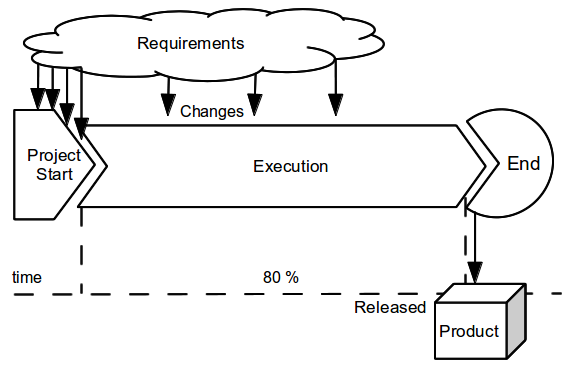
\includegraphics[width=0.8\textwidth]{PMIProject}
  \caption{Ciclo de vida en una Gestión de Proyectos tradicional}
  \centering
  \label{fig:PMIProject} %\ref{fig:PMIProject}
\end{figure}


\subsubsection{Metodología en Cascada}

La combinación del "Modelo en Cascada" con la "Gestión de Proyectos Clásica" conforma la metodología e idea de desarrollo de proyectos en forma de cascada (ver figura \ref{fig:WaterfallMethodology}). La idea se relaciona con una "carrera de relevos secuencial" en la que está incluida la administración del proyecto (proceso de gestión) y la producción del mismo (proceso de desarrollo) en una secuencia prácticamente lineal y en fases secuenciales.

\begin{figure}[h]
  \centering
  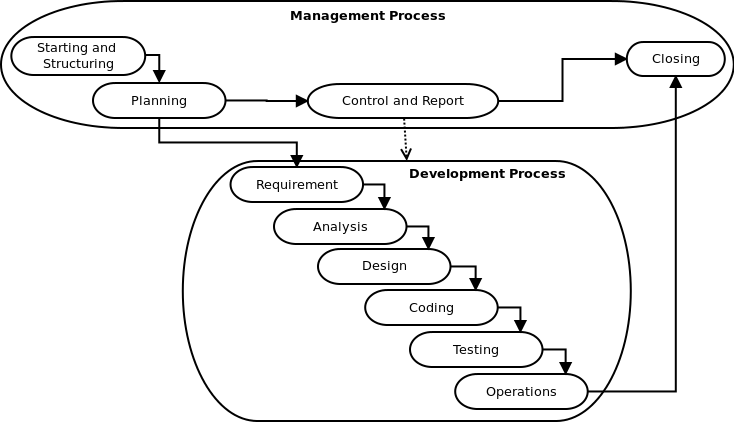
\includegraphics[width=0.99\textwidth]{WaterfallMethodology}
  \caption{Metodología Cascada criticada por Scrum}
  (Diagrama integrador del Modelo Cascada \cite{Winston-Royce-1970}, la Metodología Cascada \cite{Ken-Schwaber-1995} y la Metodología de Gestión de Proyectos \cite{PMBOK-1996})
  \centering
  \label{fig:WaterfallMethodology} %\ref{fig:WaterfallMethodology}
\end{figure}
